% This is samplepaper.tex, a sample chapter demonstrating the
% LLNCS macro package for Springer Computer Science proceedings;
% Version 2.21 of 2022/01/12
%
\documentclass[runningheads]{llncs}
%
\usepackage[T1]{fontenc}
% T1 fonts will be used to generate the final print and online PDFs,
% so please use T1 fonts in your manuscript whenever possible.
% Other font encondings may result in incorrect characters.
%
\usepackage{graphicx}
\usepackage{hyperref}
% Used for displaying a sample figure. If possible, figure files should
% be included in EPS format.
%
% If you use the hyperref package, please uncomment the following two lines
% to display URLs in blue roman font according to Springer's eBook style:
\usepackage{color}
\renewcommand\UrlFont{\color{blue}\rmfamily}
\urlstyle{rm}

\usepackage{amsmath}
\usepackage{amssymb}
\usepackage{tikz}
\usepackage{wrapfig}
\usepackage{environ}

\usepackage{changes}
\usepackage{algorithm}
\usepackage[noend]{algpseudocode}
\usepackage{varwidth}
\usepackage{mathtools}
\usepackage{pgfplots}
\usepackage[dvipsnames]{xcolor}
\pgfplotsset{compat=1.18}
\usetikzlibrary {arrows.meta,decorations.shapes}
\setauthormarkup{}
\definechangesauthor[name=jo, color=magenta]{JO}
\definechangesauthor[name=rom, color=teal]{ROM}

% set of real numbers
\newcommand{\R}{\ensuremath{\mathbb{R}}}
% set of integer numbers
\newcommand{\Z}{\ensuremath{\mathbb{Z}}}
% cell complex build on the lattice \Z^d
\let\C\relax \DeclareMathOperator{\C}{\ensuremath{\mathcal{C}^d}} % modified because of incompatiblity with hyperref package
% cardinality of a set
\newcommand{\Card}[1]{\ensuremath{\#\left( #1 \right)}}
% Interior of a closed set.
\newcommand{\Int}[1]{\ensuremath{\mathrm{Int}\left( #1 \right)}}
% Some vectors and matrices
\newcommand{\vx}[0]{\ensuremath{\mathbf{x}}}
\newcommand{\vy}[0]{\ensuremath{\mathbf{y}}}
\newcommand{\vz}[0]{\ensuremath{\mathbf{z}}}
\newcommand{\vb}[0]{\ensuremath{\mathbf{b}}}
\newcommand{\vA}[0]{\ensuremath{\mathbf{A}}}
\newcommand{\va}[0]{\ensuremath{\mathbf{a}}}
\newcommand{\vc}[0]{\ensuremath{\mathbf{c}}}
\newcommand{\ve}[0]{\ensuremath{\mathbf{e}}}
\newcommand{\vm}[0]{\ensuremath{\mathbf{m}}}
\newcommand{\vn}[0]{\ensuremath{\mathbf{n}}}
\newcommand{\vu}[0]{\ensuremath{\mathbf{u}}}
\newcommand{\vv}[0]{\ensuremath{\mathbf{v}}}
\newcommand{\vw}[0]{\ensuremath{\mathbf{w}}}
\newcommand{\vp}[0]{\ensuremath{\mathbf{p}}}
\newcommand{\vq}[0]{\ensuremath{\mathbf{q}}}
\newcommand{\vr}[0]{\ensuremath{\mathbf{r}}}
\newcommand{\vs}[0]{\ensuremath{\mathbf{s}}}
\newcommand{\vt}[0]{\ensuremath{\mathbf{t}}}
% Convex hull
\newcommand{\Conv}[1]{\mathrm{CvxH}\left( #1 \right)}

% References
\newcommand{\Equ}[1]{(\ref{#1})}
\newcommand{\RefFigure}[1]{Figure~\ref{#1}}
\newcommand{\RefLemma}[1]{Lemma~\ref{#1}}
\newcommand{\RefLemmas}[2]{Lemmas~\ref{#1} and~\ref{#2}}
\newcommand{\RefTheorem}[1]{Theorem~\ref{#1}}
\newcommand{\RefCorollary}[1]{Corollary~\ref{#1}}
\newcommand{\RefAlgorithm}[1]{Algorithm~\ref{#1}}
\newcommand{\RefSection}[1]{Section~\ref{#1}}
\newcommand{\Refline}[1]{line~\ref{#1}}
\newcommand{\RefLine}[1]{Line~\ref{#1}}

% Star, closure, boundary of a complex
\newcommand{\Bd}[1]{\ensuremath{\mathrm{Bd}\left(#1\right)}}
\newcommand{\Star}[1]{\ensuremath{\mathrm{Star}\left(#1\right)}}
\newcommand{\Starop}[0]{\ensuremath{\mathrm{Star}}}
\newcommand{\Cl}[1]{\ensuremath{\mathrm{Cl}\left(#1\right)}}
% Closed interior
\newcommand{\CI}[1]{\ensuremath{\mathrm{ClInt}\left(#1\right)}}
% Body of a complex
\newcommand{\Body}[1]{\ensuremath{\left\|#1\right\|}}
% topological closure
\newcommand{\TCl}[1]{\ensuremath{\overline{#1}}}
% topological interior
\newcommand{\TInt}[1]{\ensuremath{\mathring{#1}}}
% topological boundary
\newcommand{\TBd}[1]{\ensuremath{\partial{#1}}}
% <=
\newcommand{\Le}{\ensuremath{\leqslant}}
% >=
\newcommand{\Ge}{\ensuremath{\geqslant}}


% Euclidean distance
\newcommand{\EDist}[0]{\ensuremath{\mathrm{d}_\mathbf{E}}}
% Hausdorff distance
\newcommand{\HDist}[0]{\ensuremath{\mathrm{d}_H}}
% Normal cone to S at p
\newcommand{\NC}[2]{\ensuremath{\mathrm{N}_{#1}(#2)}}

% l2 norm
\newcommand{\ltwo}[0]{\ensuremath{\ell_2}}
\newcommand{\loo}[0]{\ensuremath{\ell_\infty}}

% Reach
\newcommand{\Reach}[1]{\ensuremath{\mathrm{reach}(#1)}}
% Volume
\newcommand{\Vol}[1]{\ensuremath{\mathrm{Vol}\left(#1\right)}}
\newcommand{\Vold}[2]{\ensuremath{\mathrm{Vol}^{#1}\left(#2\right)}}
% Digitization
\newcommand{\Dig}[2]{\ensuremath{\mathrm{D}_{#1}\left(#2\right)}}
% Counting lattice points
\newcommand{\Lat}[1]{\ensuremath{\mathcal{L}_{#1}}}
\newcommand{\LatC}[2]{\ensuremath{\Lat{#1}(#2)}}


%
\begin{document}
%
    \title{Fast and exact visibility on digitized shapes and application to saliency-aware normal estimation}
%
    \titlerunning{Fast and exact visibility on digitized shapes}
% If the paper title is too long for the running head, you can set
% an abbreviated paper title here
%
    \author{Romain Negro\inst{1}\orcidID{0000-XXXX-YYYY-ZZZZ} \and
    Jacques-Olivier Lachaud\inst{1}\orcidID{0000-0003-4236-2133}}
%
    \authorrunning{R. Negro and J.-O. Lachaud}
% First names are abbreviated in the running head.
% If there are more than two authors, 'et al.' is used.
%
    \institute{Universit\'e Savoie Mont Blanc, CNRS, LAMA, F-73000 Chambéry, France\\
    \email{\{romain.negro|jacques-olivier.lachaud\}@univ-smb.fr}}
%
    \maketitle              % typeset the header of the contribution
%
    \begin{abstract}
        Computing visibility on a geometric object requires heavy
        computations since it requires to identify pair of points that
        are visible to each other, i.e. there is a straight segment
        joining them that stays in the close vicinity of the object
        boundary. We propose to exploit a specific representation of
        digital sets based on lists of integral intervals in order to
        compute efficiently the complete visibility graph between
        lattice points of the digital shape. As a quite direct
        application, we show then how we can use visibility to estimate
        the normal vector field of a digital shape in an accurate and
        convergent manner while staying aware of the salient and sharp features of
        the shape.

        \keywords{Visibility \and Geometric inference \and Digital normal estimation \and Digital geometry}
    \end{abstract}

%%%%%%%%%%%%%%%%%%%%%%%%%%%%%%%%%%%%%%%%%%%%%%%%%%%%%%%%%%%%%%%%%%%%%%


    \section{Introduction}

    Visibility is a fundamental concept in computational geometry and
    digital topology, with applications ranging from computer vision
    (identifying occlusions) to geometric modeling (feature detection, geodesics)
    and computer graphics (path tracing, shadowmap). Visibility within
    polygons in the plane has been extensively studied in the
    litterature \cite{ghosh:2007-book} and is still studied in higher
    dimensional spaces \cite{orourke:2017-book}. The general problem
    has a high complexity. For instance, the 3d visibility complex
    between $n$ spheres and occluding spheres has a complexity
    $O(n^4)$ \cite{durand:2002-tog}. Exact 3d visibility between
    polygons and occluding polygons is often casted into 5d Euclidean
    space derived from Plücker space \cite{nirenstein:2002-ewr}, which
    nicely represents 3d lines and their respective positions. The
    computational cost remains high even with decomposition into
    coarse cells for speed up (several days of computation for a
    million triangles at the time).

    To increase efficiency, several authors have proposed to cast the
    visibility problem into a digital space, generally $\Z^3$ or its
    decomposition into cubical cells. Visibility is simplified as the
    problem if there is a connected digital straight line joining a
    pair of cells without occluding cell(s) (e.g. Soille
    \cite{soille:1994-prl} uses Bresenham line segments). Coeurjolly
    \emph{et al.} \cite{coeurjolly:2004-prl} uses a non-symmetric
    visibility definition and preimage computations to speed up that
    kind of algorithms. Chica \cite{chica:2008-spm} uses a half-cell
    erosion of the complementary space and Bresenham straight lines to
    decide visibility.
    
    We propose an algorithm that solves the following visibility
    problem: given a digital set $X \subset \Z^d$, two points $p,q$ of
    $X$ are \emph{visible} whenever the Euclidean straight line
    segment $\lbrack p,q \rbrack$ is never at chessboard distance
    ($\infty$-distance) greater or equal to $1$ from $X$.

    We focus on solving efficiently this problem because it is crucial
    in computing geometric normals along digital surfaces that are
    aware of salient features.
    
    (Work in progress)

    
    Visibility is a fundamental concept in computational geometry and digital topology, with applications ranging from computer vision to geometric modeling and computer graphics.
    In this work, we explore visibility through the lens of chord tangency, introducing a novel approach that builds on discrete geometric structures.
    Our framework leverages the discrete setting of and cell complexes, providing a rigorous foundation for analyzing visibility properties in digital spaces.


    
    We recall essential definitions from previous works, particularly the notions of cell complexes and the star operator as formalized in~\cite{lachaud:2021-dgmm} and~\cite{lachaud:2022-jmiv}.
    The integer grid serves as our primary space of study, where geometric structures are discretized using cell complexes.
    A cell complex is a decomposition of space into elementary units (vertices, edges, faces, and higher-dimensional counterparts) forming a combinatorial representation of geometric objects.
    The star of a cell, as defined in these works, consists of all higher-dimensional cells that contain it, a crucial concept for analyzing local neighborhoods and connectivity.

    Building on these foundations, our study focuses on visibility as determined by the tangency of chords in discrete geometry.
    We define and analyze how visibility relationships emerge in this context and investigate their combinatorial and topological implications.
    This approach provides a new perspective on discrete visibility, offering potential applications in digital imaging, surface reconstruction, and computational topology.

    The remainder of this paper is structured as follows.
    In Section 2, we formalize the concept of chord tangency and its role in visibility analysis.
    Section 3 enters into the usage of integer intervals intersections to quickly scan the figure in order to recover this visibiltiy.
    Section 4 presents our main results, using this visibility to compute normals using the CNC estimator~\cite{lachaud:2022-dcg}.
    Finally, Section 5 concludes with some other applications of integer intervals intersections in the field.


%%%%%%%%%%%%%%%%%%%%%%%%%%%%%%%%%%%%%%%%%%%%%%%%%%%%%%%%%%%%%%%%%%%%%%


    \section{Visibility through tangency of chords}


    Let $\Z^d$ be the d-dimensional digital space, $d$ > 0.
    Let $\mathcal{C}^d$ be the (cubical) cell complex induced by the lattice $\Z^d$ : its 0-cells are the points of $\Z^d$, its 1-cells are the open unit segments joining two 0-cells at distance 1, its 2-cells are the open unit squares, etc., and its d-cells are the d-dimensional open unit hypercubes with vertices in $\Z^d$.
    We denote $\mathcal{C}^d_k$ the set of its k-cells.
    In the following, a cell will always designate an element of $\mathcal{C}^d$, and the term subcomplex always designates a subset of $\mathcal{C}^d$.

    A cell $\sigma$ is a face of another cell $\tau$ whenever $\sigma$ is a subset of the topological closure $\bar{\tau}$ of $\tau$, written $\sigma \preccurlyeq \tau$.
    Given any subcomplex K of $\mathcal{C}^d$, the star $Star(K)$ of K is $\{\tau \in \mathcal{C}^d, s.t.\ \exists\sigma \in K,\sigma \preccurlyeq \tau\}$

    \begin{definition}
        Two points \( p \) and \( q \) on \( K \) are visible if and only if the segment \([p, q]\) is included in \(\text{Star}(K)\), i.e., \( [p, q] \subseteq \text{Star}(K)\)
    \end{definition}

    % Examples of visibility in 2D
    \begin{figure}
        \centering
        \begin{tabular}{cc|cc}
            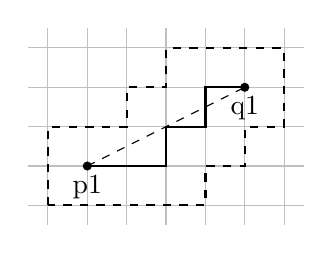
\begin{tikzpicture}
                \draw[step=0.5,lightgray,thin,xshift=-1cm,yshift=-1cm] (0.25,0.25) grid (3.75,2.75);
                \draw[dashed] (0,0) -- (2,1);
                \filldraw[black] (0,0) circle (0.05) node[anchor=north] {p1};
                \filldraw[black] (2,1) circle (0.05) node[anchor=north] {q1};
                \draw [thick] (0,0) -- (0.5,0) -- (1,0) -- (1,0.5) -- (1.5,0.5) -- (1.5,1) -- (2,1);
                \draw[thick,dashed] (-0.5,-0.5) -- (-0.5,0.5) -- (0.5,0.5) -- (0.5,1) -- (1,1) -- (1,1.5) -- (2.5,1.5) -- (2.5,0.5) -- (2,0.5) -- (2,0) -- (1.5,0) -- (1.5,-0.5) -- (-0.5,-0.5);
            \end{tikzpicture} & & &
            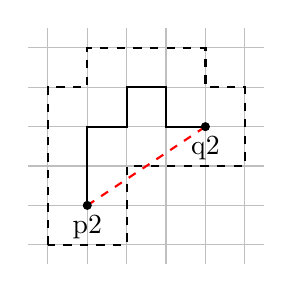
\begin{tikzpicture}
                \draw[step=0.5,lightgray,thin,xshift=-1cm,yshift=-1cm] (0.25,0.25) grid (3.25,3.25);
                \draw[red,dashed,thick] (0,0) -- (1.5,1);
                \filldraw[black] (0,0) circle (0.05) node[anchor=north] {p2};
                \filldraw[black] (1.5,1) circle (0.05) node[anchor=north] {q2};
                \draw [thick] (0,0) -- (0,1) -- (0.5,1) -- (0.5,1.5) -- (1,1.5) -- (1,1) -- (1.5,1);
                \draw[thick,dashed] (-0.5,-0.5) -- (-0.5,1.5) -- (0,1.5) -- (0,2) -- (1.5,2) -- (1.5,1.5) -- (2,1.5)  -- (2,0.5) -- (0.5,0.5) -- (0.5,-0.5) -- (-0.5,-0.5);
            \end{tikzpicture} \\
            Visible                       & & & Non Visible                   \\\\
            \hline\\
            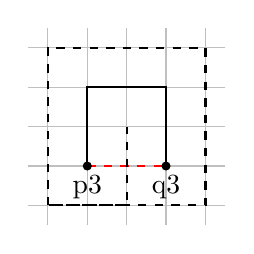
\begin{tikzpicture}
                \draw[step=0.5,lightgray,thin,xshift=-1cm,yshift=-1cm] (0.25,0.25) grid (2.75,2.75);
                \draw[red,dashed,thick] (0,0) -- (1,0);
                \filldraw[black] (0,0) circle (0.05) node[anchor=north] {p3};
                \filldraw[black] (1,0) circle (0.05) node[anchor=north] {q3};
                \draw [thick] (0,0) -- (0,1) -- (1,1) -- (1,0);
                \draw[thick,dashed] (-0.5,-0.5) -- (-0.5,1.5) -- (1.5,1.5) -- (1.5,-0.5) -- (-0.5,-0.5) -- (0.5,-0.5) -- (0.5,0.5);
            \end{tikzpicture} & & &
            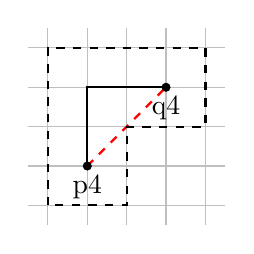
\begin{tikzpicture}
                \draw[step=0.5,lightgray,thin,xshift=-1cm,yshift=-1cm] (0.25,0.25) grid (2.75,2.75);
                \draw[red,dashed,thick] (0,0) -- (1,1);
                \filldraw[black] (0,0) circle (0.05) node[anchor=north] {p4};
                \filldraw[black] (1,1) circle (0.05) node[anchor=north] {q4};
                \draw [thick] (0,0) -- (0,1) -- (1,1);
                \draw[thick,dashed] (-0.5,-0.5) -- (-0.5,1.5) -- (1.5,1.5) -- (1.5,0.5) -- (0.5,0.5) -- (0.5,-0.5) -- (-0.5,-0.5);
            \end{tikzpicture}\\
            Non Visible (from a 1-d cell) & & & Non Visible (from a 0-d cell)
        \end{tabular}
        \caption{Examples of visibility in 2D.}
        \label{fig:visibility-2d}
    \end{figure}


    We note that one particular aspect of this visibility definition is that all visible points from a given point taken as a separate complex are not necessarily 26-connected~\ref{fig:visibility-2d-not-connected}.
    Furthermore, we conjecture that they even may not be $n$-connected for $n$ arbitrarily large.
    This characteristic has implications for the applicability of Algorithm 3 from~\cite{lachaud:2022-jmiv}, as the algorithm assumes that visited points are 26-connected, potentially leading to incomplete collection of visible points.

    % Example of visibility not necessarily connected
    % Path from p to q : r u r u r r r r r u r
    \begin{figure}
        \centering
        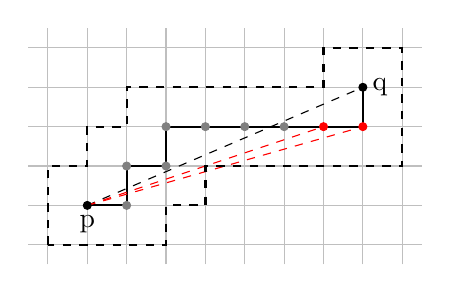
\begin{tikzpicture}
            \draw[step=0.5,lightgray,thin,xshift=-1cm,yshift=-1cm] (0.25,0.25) grid (5.25,3.25);
            \draw[thick] (0,0) -- (0.5,0) -- (0.5,0.5) -- (1,0.5) -- (1,1) -- (3.5,1) -- (3.5,1.5);
            \draw [black, dashed] (0,0) -- (3.5,1.5);
            \draw [red, dashed] (0,0) -- (3.5,1);
            \draw [red, dashed] (0,0) -- (3,1);
            \filldraw[black] (0,0) circle (0.05) node[anchor=north] {p};
            \filldraw[gray] (0.5,0) circle (0.05);
            \filldraw[gray] (0.5,0.5) circle (0.05);
            \filldraw[gray] (1,0.5) circle (0.05);
            \filldraw[gray] (1,1) circle (0.05);
            \filldraw[gray] (1.5,1) circle (0.05);
            \filldraw[gray] (2,1) circle (0.05);
            \filldraw[gray] (2.5,1) circle (0.05);
            \filldraw[red] (3,1) circle (0.05);
            \filldraw[red] (3.5,1) circle (0.05);
            \filldraw[black] (3.5,1.5) circle (0.05) node[anchor=west] {q};
            \draw[thick,dashed] (-0.5,-0.5) -- (-0.5,0.5) -- (0,0.5) -- (0,1) -- (0.5,1) -- (0.5,1.5) -- (3,1.5) -- (3,2) -- (4,2) -- (4,0.5) -- (1.5,0.5) -- (1.5,0) -- (1,0) -- (1,-0.5) -- (-0.5,-0.5);
        \end{tikzpicture}
        \caption{Example of non-connex visibility in 2D, q is visible from p while the visibility points are not 26-connected.}
        \label{fig:visibility-2d-not-connected}
    \end{figure}

%%%%%%%%%%%%%%%%%%%%%%%%%%%%%%%%%%%%%%%%%%%%%%%%%%%%%%%%%%%%%%%%%%%%%%


    \section{Fast computation using integer intervals intersections}

    To improve computation time, we will use lattice maps of integer intervals.

    \begin{definition}
        A sequence of intervals is an ordered list of intervals $L = ([a_i,b_i])_{i=1,\ldots,n}$ such that $b_i + 1 < a_{i+1}$, i.e., disjoint intervals with at least a missing integer.
    \end{definition}

    \begin{definition}
        A translation of an interval $A$ is defined as $A+t \coloneqq [a+t, b+t]$
    \end{definition}

    \begin{definition}
        A translation of a sequence of intervals $L$ is the sequence defined as $L+t \coloneqq \{L_1+t,\ldots,L_n+t\}$
    \end{definition}

    \begin{definition}
        All translations $T$ of an interval or a sequence of intervals $A$ in a sequence of intervals $L$ are defined as $ T \coloneqq \{ t, st. A+t \subset L\}$
    \end{definition}

    We will consider lattice maps as pairs of (shift, intervals), where shifts are points $p \in \R^{d-1}$. All coordinates are doubled, so that the represented cell $\forall c \in \R^d$ will have a dimension equal to $\sum_{i=1}^d \left(c[i]\mod d\right)$. Note that all examples are in 2-d while the shown algorithm is in n-d.

    \begin{figure}
        \centering
        \label{fig:lattice-representation}
        % \usetikzlibrary {arrows.meta,decorations.shapes}
        \begin{tabular}{c c}
            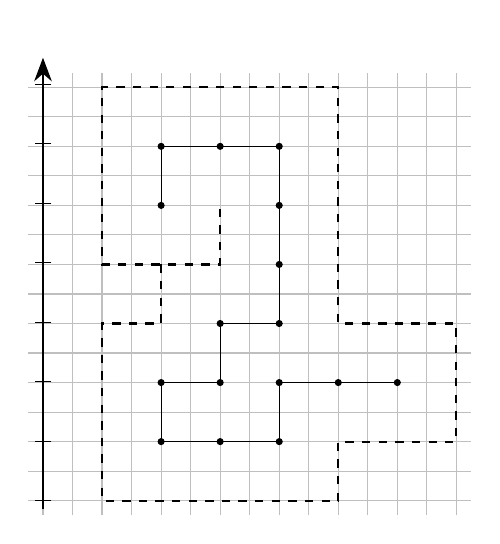
\begin{tikzpicture}[scale=0.75]
                \draw[step=0.5,lightgray,thin,xshift=-1cm,yshift=-1cm] (-0.25,-0.25) grid (7.25,7.25);
                \filldraw[black] (1,4) circle (0.05);
                \filldraw[black] (1,5) circle (0.05);
                \filldraw[black] (2,5) circle (0.05);
                \filldraw[black] (3,5) circle (0.05);
                \filldraw[black] (3,4) circle (0.05);
                \filldraw[black] (3,3) circle (0.05);
                \filldraw[black] (3,2) circle (0.05);
                \filldraw[black] (2,2) circle (0.05);
                \filldraw[black] (2,1) circle (0.05);
                \filldraw[black] (1,1) circle (0.05);
                \filldraw[black] (1,0) circle (0.05);
                \filldraw[black] (2,0) circle (0.05);
                \filldraw[black] (3,0) circle (0.05);
                \filldraw[black] (3,1) circle (0.05);
                \filldraw[black] (4,1) circle (0.05);
                \filldraw[black] (5,1) circle (0.05);
                \draw[-{Stealth[length=3mm]}=black] (-1,-1) -- (-1,6.5);
                \draw decorate [decoration={crosses,transform={rotate=45},shape size=1.5mm,segment length=21.5pt}] {(-1,-1) -- (-1,7)};
                \draw[black] (1,4) -- (1,5) -- (3,5) -- (3,2) -- (2,2) -- (2,1) -- (1,1) -- (1,0) -- (3,0) -- (3,1) -- (5,1);
                \draw[thick,dashed] (1,3) -- (1,2) -- (0,2) -- (0,-1) -- (4,-1) -- (4,0) -- (6,0) -- (6,2) -- (4,2) -- (4,6) -- (0,6) -- (0,3) -- (2,3) -- (2,4);
            \end{tikzpicture} &
            %      \begin{tikzpicture}
            %     \foreach \y in {1,1.5,...,6} {
            %       \draw[thin, lightgray,xshift=-1cm,yshift=-1cm] (0.75,\y) -- (6.25,\y);
            %     }
            %     \draw[-{Stealth[length=3mm]}=black] (0,0) -- (0,5.5);
            %     \draw decorate [decoration={crosses,transform={rotate=45},shape size=1.5mm,segment length=10mm}] {(0,0) -- (0,5)};
            %     \draw[black] (1,4) -- (1,5) -- (3,5) -- (3,2) -- (2,2) -- (2,1) -- (1,1) -- (1,0) -- (3,0) -- (3,1) -- (5,1);
            %     \draw[thick, arrows = {Bracket[sharp]-Bracket[sharp]}] (0.9,5)--(3.1,5);
            %     \draw[thick, arrows = {Bracket[sharp]-Bracket[sharp]}] (0.9,4.5)--(1.1,4.5);
            %     \draw[thick, arrows = {Bracket[sharp]-Bracket[sharp]}] (2.9,4.5)--(3.1,4.5);
            %     \draw[thick, arrows = {Bracket[sharp]-Bracket[sharp]}] (0.9,4)--(1.1,4);
            %     \draw[thick, arrows = {Bracket[sharp]-Bracket[sharp]}] (2.9,4)--(3.1,4);
            %     \draw[thick, arrows = {Bracket[sharp]-Bracket[sharp]}] (2.9,3.5)--(3.1,3.5);
            %     \draw[thick, arrows = {Bracket[sharp]-Bracket[sharp]}] (2.9,3)--(3.1,3);
            %     \draw[thick, arrows = {Bracket[sharp]-Bracket[sharp]}] (2.9,2.5)--(3.1,2.5);
            %     \draw[thick, arrows = {Bracket[sharp]-Bracket[sharp]}] (1.9,2)--(3.1,2);
            %     \draw[thick, arrows = {Bracket[sharp]-Bracket[sharp]}] (1.9,1.5)--(2.1,1.5);
            %     \draw[thick, arrows = {Bracket[sharp]-Bracket[sharp]}] (0.9,1)--(2.1,1);
            %     \draw[thick, arrows = {Bracket[sharp]-Bracket[sharp]}] (2.9,1)--(5.1,1);
            %     \draw[thick, arrows = {Bracket[sharp]-Bracket[sharp]}] (0.9,0.5)--(1.1,0.5);
            %     \draw[thick, arrows = {Bracket[sharp]-Bracket[sharp]}] (2.9,0.5)--(3.1,0.5);
            %     \draw[thick, arrows = {Bracket[sharp]-Bracket[sharp]}] (0.9,0)--(3.1,0);
            %     \filldraw[white,yshift=-1cm] (0,0) circle (0.01); % readjust the height to match the original path
            % \end{tikzpicture} &
            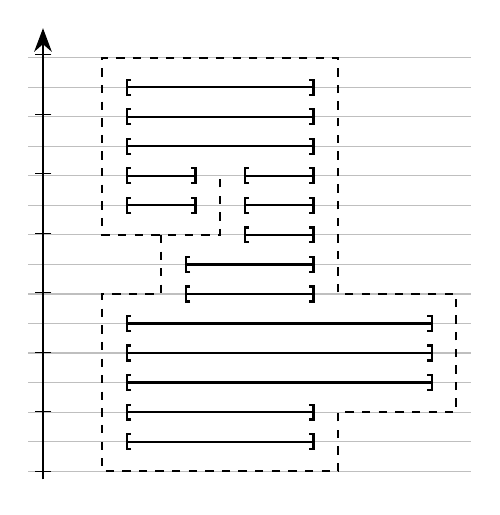
\begin{tikzpicture}[scale=0.75]
                \foreach \y in {0,0.5,...,7} {
                    \draw[thin, lightgray,xshift=-1cm,yshift=-1cm] (-0.25,\y) -- (7.25,\y);
                }
                \draw[-{Stealth[length=3mm]}=black] (-1,-1) -- (-1,6.5);
                \draw decorate [decoration={crosses,transform={rotate=45},shape size=1.5mm,segment length=21.5pt}] {(-1,-1) -- (-1,6.5)};
                \draw[thick,dashed] (1,3) -- (1,2) -- (0,2) -- (0,-1) -- (4,-1) -- (4,0) -- (6,0) -- (6,2) -- (4,2) -- (4,6) -- (0,6) -- (0,3) -- (2,3) -- (2,4);
                \draw[thick, arrows = {Bracket[sharp]-Bracket[sharp]}] (0.4,5.5)--(3.6,5.5);
                \draw[thick, arrows = {Bracket[sharp]-Bracket[sharp]}] (0.4,5)--(3.6,5);
                \draw[thick, arrows = {Bracket[sharp]-Bracket[sharp]}] (0.4,4.5)--(3.6,4.5);
                \draw[thick, arrows = {Bracket[sharp]-Bracket[sharp]}] (0.4,4)--(1.6,4);
                \draw[thick, arrows = {Bracket[sharp]-Bracket[sharp]}] (2.4,4)--(3.6,4);
                \draw[thick, arrows = {Bracket[sharp]-Bracket[sharp]}] (0.4,3.5)--(1.6,3.5);
                \draw[thick, arrows = {Bracket[sharp]-Bracket[sharp]}] (2.4,3.5)--(3.6,3.5);
                \draw[thick, arrows = {Bracket[sharp]-Bracket[sharp]}] (2.4,3)--(3.6,3);
                \draw[thick, arrows = {Bracket[sharp]-Bracket[sharp]}] (1.4,2.5)--(3.6,2.5);
                \draw[thick, arrows = {Bracket[sharp]-Bracket[sharp]}] (1.4,2)--(3.6,2);
                \draw[thick, arrows = {Bracket[sharp]-Bracket[sharp]}] (0.4,1.5)--(5.6,1.5);
                \draw[thick, arrows = {Bracket[sharp]-Bracket[sharp]}] (0.4,1)--(5.6,1);
                \draw[thick, arrows = {Bracket[sharp]-Bracket[sharp]}] (0.4,0.5)--(5.6,0.5);
                \draw[thick, arrows = {Bracket[sharp]-Bracket[sharp]}] (0.4,0)--(3.6,0);
                \draw[thick, arrows = {Bracket[sharp]-Bracket[sharp]}] (0.4,-0.5)--(3.6,-0.5);
                \filldraw[white,yshift=-1.25cm] (0,0) circle (0.01); % readjust the height to match the original path
            \end{tikzpicture}
        \end{tabular}
        \caption{Representation of a 2d cell complex (here the star of a given curve) as a lattice map. From 31 cells from the star on the left, we get 15 intervals on the right}
    \end{figure}

    \colorlet{MyGreen}{green!80!gray}
    \begin{figure}
        \centering
        \begin{tabular}{c c}
            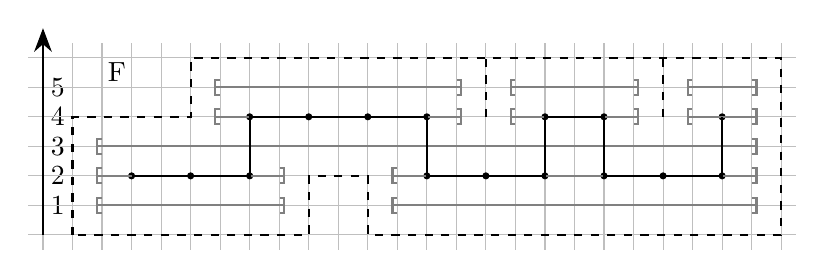
\begin{tikzpicture}[scale=0.75]
                \foreach[count=\i] \y in {-0.5,0,...,1.5} {
                    \draw (0,0) node at (-1.25,\y) {\i};
                }
                \draw[step=0.5,lightgray,thin,xshift=-1cm,yshift=-1cm] (-0.75,-0.25) grid (12.25,3.25);
                \draw[-{Stealth[length=3mm]}=black] (-1.5,-1) -- (-1.5,2.5);
                \filldraw[black] (0,0) circle (0.05);
                \filldraw[black] (1,0) circle (0.05);
                \filldraw[black] (2,0) circle (0.05);
                \filldraw[black] (2,1) circle (0.05);
                \filldraw[black] (3,1) circle (0.05);
                \filldraw[black] (4,1) circle (0.05);
                \filldraw[black] (5,1) circle (0.05);
                \filldraw[black] (5,0) circle (0.05);
                \filldraw[black] (6,0) circle (0.05);
                \filldraw[black] (7,0) circle (0.05);
                \filldraw[black] (7,1) circle (0.05);
                \filldraw[black] (8,1) circle (0.05);
                \filldraw[black] (8,0) circle (0.05);
                \filldraw[black] (9,0) circle (0.05);
                \filldraw[black] (10,0) circle (0.05);
                \filldraw[black] (10,1) circle (0.05);
                \draw[thick,gray, arrows = {Bracket[sharp]-Bracket[sharp]}] (-0.6,-0.5)--(2.6,-0.5);
                \draw[thick,gray, arrows = {Bracket[sharp]-Bracket[sharp]}] (4.4,-0.5)--(10.6,-0.5);
                \draw[thick,gray, arrows = {Bracket[sharp]-Bracket[sharp]}] (-0.6,0)--(2.6,0);
                \draw[thick,gray, arrows = {Bracket[sharp]-Bracket[sharp]}] (4.4,0)--(10.6,0);
                \draw[thick,gray, arrows = {Bracket[sharp]-Bracket[sharp]}] (-0.6,0.5)--(10.6,0.5);
                \draw[thick,gray, arrows = {Bracket[sharp]-Bracket[sharp]}] (1.4,1)--(5.6,1);
                \draw[thick,gray, arrows = {Bracket[sharp]-Bracket[sharp]}] (6.4,1)--(8.6,1);
                \draw[thick,gray, arrows = {Bracket[sharp]-Bracket[sharp]}] (9.4,1)--(10.6,1);
                \draw[thick,gray, arrows = {Bracket[sharp]-Bracket[sharp]}] (1.4,1.5)--(5.6,1.5);
                \draw[thick,gray, arrows = {Bracket[sharp]-Bracket[sharp]}] (6.4,1.5)--(8.6,1.5);
                \draw[thick,gray, arrows = {Bracket[sharp]-Bracket[sharp]}] (9.4,1.5)--(10.6,1.5);
                \draw[thick, black] (0,0) -- (2,0) -- (2,1) -- (5,1) -- (5,0) -- (7,0) -- (7,1) -- (8,1) -- (8,0) -- (10,0) -- (10,1);
                \draw[thick,dashed] (6,1) -- (6,2);
                \draw[thick,dashed] (9,1) -- (9,2);
                \draw[thick,dashed] (-1,-1) -- (-1,1) -- (1,1) -- (1,2) -- (11,2) -- (11,-1) -- (4,-1) -- (4,0) -- (3,0) -- (3,-1) -- (-1,-1);

                \draw (0,0) node at (-0.25,1.75) {F};

            \end{tikzpicture} &
            \begin{tikzpicture}[scale=0.75]
                \draw[step=0.5,lightgray,thin,xshift=-1cm,yshift=-1cm] (-0.75,-0.25) grid (4.25,3.25);
                \draw[-{Stealth[length=3mm]}=black] (-1.5,-1) -- (-1.5,2.5);
                \foreach[count=\i] \y in {-0.5,0,...,1.5} {
                    \draw (0,0) node at (-1.25,\y) {\i};
                }
                \filldraw[black] (0,0) circle (0.05);
                \filldraw[black] (2,1) circle (0.05);
                \draw[thick, black] (0,0) -- (2,1);
                \draw[thick,dashed] (-1,-1) -- (-1,1) -- (1,1) -- (1,2) -- (3,2) -- (3,0) -- (1,0) --  (1,-1) -- (-1,-1);
                \draw[thick,MyGreen, arrows = {Bracket[sharp]-Bracket[sharp]}] (-0.6,-0.5)--(0.6,-0.5);
                \draw[thick,MyGreen, arrows = {Bracket[sharp]-Bracket[sharp]}] (-0.6,0)--(0.6,0);
                \draw[thick,MyGreen, arrows = {Bracket[sharp]-Bracket[sharp]}] (-0.6,0.5)--(2.6,0.5);
                \draw[thick,MyGreen, arrows = {Bracket[sharp]-Bracket[sharp]}] (1.4,1)--(2.6,1);
                \draw[thick,MyGreen, arrows = {Bracket[sharp]-Bracket[sharp]}] (1.4,1.5)--(2.6,1.5);

                \draw (0,0) node at (-0.25,1.75) {V};
            \end{tikzpicture}\\
            \hline
            \multicolumn{2}{c}{
                \begin{tikzpicture}[scale=0.75]
                    \foreach \y in {0,0.5,...,12.5} {
                        \draw[thin, lightgray] (-1.25,\y) -- (11.25,\y);
                    }
                    \foreach \y in {0,2.5,...,12.5} {
                        \draw[blue] (-7,\y) -- (11.25,\y);
                    }

                    \foreach[count=\i] \y in {12,9.5,...,2} {
                        \draw (0,0) node at (-4,\y) {$V_{\i}$};
                    }
                    \foreach[count=\i] \y in {11.5,9,...,1.5} {
                        \draw (0,0) node at (-4,\y) {$F_{\i}$};
                    }
                    \draw (0,0) node at (-4,11) {$T_{1} = \text{Translations}(V_{1},F_{1})$};
                    \foreach[count=\i] \y in {8.5,6,...,1} {
                        \draw (0,0) node at (-4,\y) {$T_{\the\numexpr\i+1\relax}$};
                    }
                    \draw (0,0) node at (-4,10.5) {$R_1 = T_1$};

                    \foreach[count=\i] \y in {8,5.5,...,0.5} {

                        \draw (0,0) node at (-4,\y) {$R_{\the\numexpr\i+1\relax} = T_{\the\numexpr\i+1\relax} \cap R_{\i}$};
                    }

                    \draw[thick,MyGreen,arrows = {Bracket[sharp]-Bracket[sharp]}] (-0.6,12)--(0.6,12);
                    \draw[thick,gray,arrows = {Bracket[sharp]-Bracket[sharp]}] (-0.6,11.5)--(2.6,11.5);
                    \draw[thick,gray,arrows = {Bracket[sharp]-Bracket[sharp]}] (4.4,11.5)--(10.6,11.5);
                    \draw[thick,violet,arrows = {Bracket[sharp]-Bracket[sharp]}] (-0.6,11)--(1.6,11);
                    \draw[thick,violet,arrows = {Bracket[sharp]-Bracket[sharp]}] (4.4,11)--(9.6,11);
                    \draw[thick,red,arrows = {Bracket[sharp]-Bracket[sharp]}] (-0.6,10.5)--(1.6,10.5);
                    \draw[thick,red,arrows = {Bracket[sharp]-Bracket[sharp]}] (4.4,10.5)--(9.6,10.5);

                    \draw[thick,MyGreen,arrows = {Bracket[sharp]-Bracket[sharp]}] (-0.6,9.5)--(0.6,9.5);
                    \draw[thick,gray,arrows = {Bracket[sharp]-Bracket[sharp]}] (-0.6,9)--(2.6,9);
                    \draw[thick,gray,arrows = {Bracket[sharp]-Bracket[sharp]}] (4.4,9)--(10.6,9);
                    \draw[thick,violet,arrows = {Bracket[sharp]-Bracket[sharp]}] (-0.6,8.5)--(1.6,8.5);
                    \draw[thick,violet,arrows = {Bracket[sharp]-Bracket[sharp]}] (4.4,8.5)--(9.6,8.5);
                    \draw[thick,red,arrows = {Bracket[sharp]-Bracket[sharp]}] (-0.6,8)--(1.6,8);
                    \draw[thick,red,arrows = {Bracket[sharp]-Bracket[sharp]}] (4.4,8)--(9.6,8);

                    \draw[thick,MyGreen,arrows = {Bracket[sharp]-Bracket[sharp]}] (-0.6,7)--(2.6,7);
                    \draw[thick,gray,arrows = {Bracket[sharp]-Bracket[sharp]}] (-0.6,6.5)--(10.6,6.5);
                    \draw[thick,violet,arrows = {Bracket[sharp]-Bracket[sharp]}] (-0.6,6)--(7.6,6);
                    \draw[thick,red,arrows = {Bracket[sharp]-Bracket[sharp]}] (-0.6,5.5)--(1.6,5.5);
                    \draw[thick,red,arrows = {Bracket[sharp]-Bracket[sharp]}] (4.4,5.5)--(7.6,5.5);

                    \draw[thick,black,arrows = {-Stealth[]}] (-0.6,4.5)--(1.4,4.5);
                    \draw[thick,MyGreen,arrows = {Bracket[sharp]-Bracket[sharp]}] (1.4,4.5)--(2.6,4.5);
                    \draw[thick,gray,arrows = {Bracket[sharp]-Bracket[sharp]}] (1.4,4)--(5.6,4);
                    \draw[thick,gray,arrows = {Bracket[sharp]-Bracket[sharp]}] (6.4,4)--(8.6,4);
                    \draw[thick,gray,arrows = {Bracket[sharp]-Bracket[sharp]}] (9.4,4)--(10.6,4);
                    \draw[thick,violet,arrows = {Bracket[sharp]-Bracket[sharp]}] (-0.6,3.5)--(2.6,3.5);
                    \draw[thick,violet,arrows = {Bracket[sharp]-Bracket[sharp]}] (4.4,3.5)--(5.6,3.5);
                    \draw[thick,violet,arrows = {Bracket[sharp]-Bracket[sharp]}] (7.4,3.5)--(7.6,3.5);
                    \draw[thick,red,arrows = {Bracket[sharp]-Bracket[sharp]}] (-0.6,3)--(1.6,3);
                    \draw[thick,red,arrows = {Bracket[sharp]-Bracket[sharp]}] (4.4,3)--(5.6,3);
                    \draw[thick,red,arrows = {Bracket[sharp]-Bracket[sharp]}] (7.4,3)--(7.6,3);

                    \draw[thick,black,arrows = {-Stealth[]}] (-0.6,2)--(1.4,2);
                    \draw[thick,MyGreen,arrows = {Bracket[sharp]-Bracket[sharp]}] (1.4,2)--(2.6,2);
                    \draw[thick,gray,arrows = {Bracket[sharp]-Bracket[sharp]}] (1.4,1.5)--(5.6,1.5);
                    \draw[thick,gray,arrows = {Bracket[sharp]-Bracket[sharp]}] (6.4,1.5)--(8.6,1.5);
                    \draw[thick,gray,arrows = {Bracket[sharp]-Bracket[sharp]}] (9.4,1.5)--(10.6,1.5);
                    \draw[thick,violet,arrows = {Bracket[sharp]-Bracket[sharp]}] (-0.6,1)--(2.6,1);
                    \draw[thick,violet,arrows = {Bracket[sharp]-Bracket[sharp]}] (4.4,1)--(5.6,1);
                    \draw[thick,violet,arrows = {Bracket[sharp]-Bracket[sharp]}] (7.4,1)--(7.6,1);
                    \draw[thick,red,arrows = {Bracket[sharp]-Bracket[sharp]}] (-0.6,0.5)--(1.6,0.5);
                    \draw[thick,red,arrows = {Bracket[sharp]-Bracket[sharp]}] (4.4,0.5)--(5.6,0.5);
                    \draw[thick,red,arrows = {Bracket[sharp]-Bracket[sharp]}] (7.4,0.5)--(7.6,0.5);

                \end{tikzpicture}}
        \end{tabular}
        \caption{Evolution of the visibility check algorithm for a 2,1 vector. Green is the vector lattice map, black is the figure lattice map, red are the current intervals of positions where the visibility is still possible. The last red intervals are the visible positions. We travel the lattice maps from bottom-up. }
        \label{fig:enter-label}
    \end{figure}

    \begin{algorithm}
        \caption{Given a cell complex C and a radius $r$, compute the visibility at every point of C up to distance $r$. We assume z being the main axis of the lattice maps, x and y being the auxiliary axises}
        \label{alg:visibility}
        \begin{algorithmic}
            \Function{Visibility}{C: Cell complex, r: Integer}
                \State $\Omega \gets \Call{Star}{C}$ \Comment{Lattice map of the star of the studied cell complex}
                \State $Directions \gets \Call{GetAllPrimalDirections}{r}$
                \State $V: \text{vector of boolean} \gets [0, \ldots, 0]$ \Comment{length $Size(Directions) \times \#C.pointels$}
                \State $low, high \gets \Call{BoundingBoxZ}{\Omega}$
                \ForAll{$d$ in $Directions$}
                    \ForAll{shift $S$ in $\Omega$}
                        \State $R \gets [low, high]$
                        \ForAll{pair $P$ in $\Call{Star}{\text{d}}$}
                            \State $R \gets R \cap \Call{Translations}{P.intervals,\Omega[S + P.shift]}$
                        \EndFor
                        \State \Call{UpdateVisibility}{$V$, $R$}
                    \EndFor
                \EndFor
                \State \Return $V$
            \EndFunction
        \end{algorithmic}
    \end{algorithm}

    \begin{algorithm}
        \caption{Given 2 lists of intervals $K$ and $L$, find $K \cap L$, the intersection of those 2 lists}
        \label{alg:intersection}
        \begin{algorithmic}
            \Function{Intersection ($\cap$)}{\text{K, L}: Intervals}
                \State $R \gets \emptyset$; $k, l \gets 0$
                \While{$k < K.nbIntervals \And l < L.nbIntervals$}
                    \State $[a,b] \gets K[k]$; $[c,d] \gets L[l]$
                    \State $e \gets \max(a, c)$; $f \gets \min(b, d)$
                    \If{$e \leq f$}
                        \State $R.append([e, f])$
                    \EndIf
                    \If{$b \leq d$}
                        \State $k \gets k+1$
                    \EndIf
                    \If{$d \leq b$}
                        \State $l \gets l+1$
                    \EndIf
                \EndWhile
                \State \Return $R$
            \EndFunction
        \end{algorithmic}
    \end{algorithm}

%%%%%%%%%%%%%%%%%%%%%%%%%%%%%%%%%%%%%%%%%%%%%%%%%%%%%%%%%%%%%%%%%%%%%%


    \section{Feature-aware normal estimation on digital surfaces}

    \pgfplotsset{width=13cm}
    \begin{figure}
        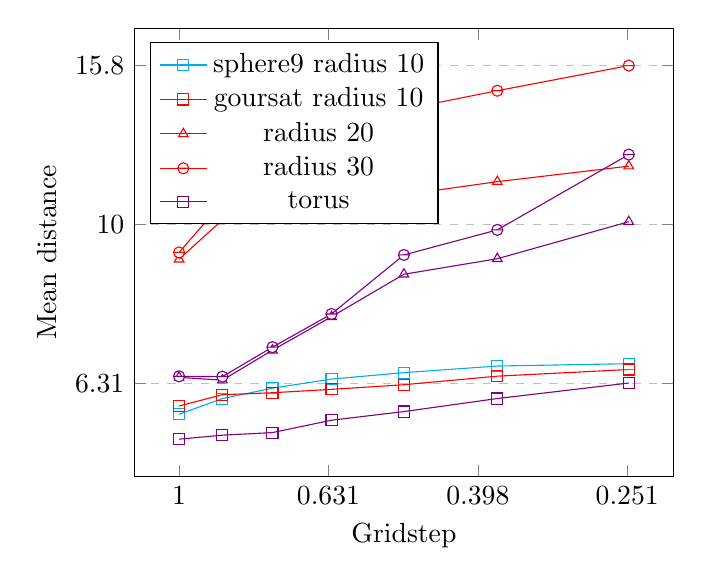
\begin{tikzpicture}
            \centering
            \begin{axis}[
                xlabel={Gridstep},
                x dir=reverse,
                ylabel={Mean distance},
                legend pos=north west,
                ymajorgrids=true,
                grid style=dashed,
                ymode=log,
                xmode=log,
                log ticks with fixed point,
            ]

                \addplot[
                    color=cyan,
                    mark=square,
                ]
                coordinates {
                    (1,5.76973)(0.875,6.03836)(0.75,6.22426)(0.625,6.39012)(0.5,6.51014)(0.375,6.63571)(0.25,6.68132)
                };
                \addlegendentry{sphere9 radius 10}
                \addplot[
                    color=red,
                    mark=square,
                ]
                coordinates {
                    (1,5.91022)(0.875,6.10641)(0.75,6.14175)(0.625,6.20202)(0.5,6.28637)(0.375,6.44418)(0.25,6.56938)
                };
                \addlegendentry{goursat radius 10}
                \addplot[
                    color=red,
                    mark=triangle,
                ]
                coordinates {
                    (1,9.04228)(0.875,10.1319)(0.75,10.2837)(0.625,10.6125)(0.5,10.8969)(0.375,11.3186)(0.25,11.8382)
                };
                \addlegendentry{radius 20}
                \addplot[
                    color=red,
                    mark=halfcircle,
                ]
                coordinates {
                    (1,9.22083)(0.875,10.6476)(0.75,11.5976)(0.625,12.7428)(0.5,13.9534)(0.375,14.73)(0.25,15.8425)
                };
                \addlegendentry{radius 30}
                \addplot[
                    color=violet,
                    mark=square,
                ]
                coordinates {
                    (1,5.36873)(0.875,5.43148)(0.75,5.47206)(0.625,5.67227)(0.5,5.81554)(0.375,6.03961)(0.25,6.31671)
                };
                \addlegendentry{torus}
                \addplot[
                    color=violet,
                    mark=triangle,
                ]
                coordinates {
                    (1,6.42158)(0.875,6.36929)(0.75,6.94675)(0.625,7.65529)(0.5,8.65652)(0.375,9.05402)(0.25,10.0784)
                };
                \addplot[
                    color=violet,
                    mark=halfcircle,
                ]
                coordinates {
                    (1,6.44119)(0.875,6.43563)(0.75,7.00852)(0.625,7.71613)(0.5,9.1544)(0.375,9.84299)(0.25,12.241)
                };
            \end{axis}
        \end{tikzpicture}
        \caption{Mean Visibility Distance as a Function of Grid Resolution}
    \end{figure}
    \begin{figure}
        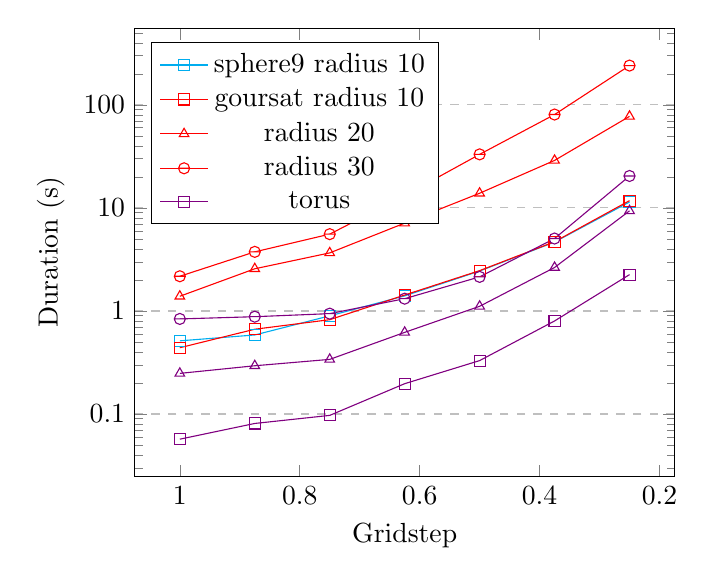
\begin{tikzpicture}
            \centering
            \begin{axis}[
                xlabel={Gridstep},
                x dir=reverse,
                ylabel={Duration (s)},
                legend pos=north west,
                ymajorgrids=true,
                grid style=dashed,
                ymode=log,
                log ticks with fixed point,
            ]

                \addplot[
                    color=cyan,
                    mark=square,
                ]
                coordinates {
                    (1,0.513)(0.875,0.585)(0.75,0.897)(0.625,1.401)(0.5,2.441)(0.375,4.664)(0.25,11.420)
                };
                \addlegendentry{sphere9 radius 10}
                \addplot[
                    color=red,
                    mark=square,
                ]
                coordinates {
                    (1,0.440)(0.875,0.665)(0.75,0.823)(0.625,1.428)(0.5,2.463)(0.375,4.697)(0.25,11.766)
                };
                \addlegendentry{goursat radius 10}
                \addplot[
                    color=red,
                    mark=triangle,
                ]
                coordinates {
                    (1,1.389)(0.875,2.567)(0.75,3.661)(0.625,7.123)(0.5,13.881)(0.375,28.913)(0.25,77.360)
                };
                \addlegendentry{radius 20}
                \addplot[
                    color=red,
                    mark=halfcircle,
                ]
                coordinates {
                    (1,2.172)(0.875,3.747)(0.75,5.565)(0.625,13.180)(0.5,33.088)(0.375,80.584)(0.25,240.546)
                };
                \addlegendentry{radius 30}
                \addplot[
                    color=violet,
                    mark=square,
                ]
                coordinates {
                    (1,0.057)(0.875,0.081)(0.75,0.097)(0.625,0.197)(0.5,0.330)(0.375,0.800)(0.25,2.253)
                };
                \addlegendentry{torus}
                \addplot[
                    color=violet,
                    mark=triangle,
                ]
                coordinates {
                    (1,0.248)(0.875,0.294)(0.75,0.339)(0.625,0.620)(0.5,1.110)(0.375,2.643)(0.25,9.369)
                };
                \addplot[
                    color=violet,
                    mark=halfcircle,
                ]
                coordinates {
                    (1,0.837)(0.875,0.880)(0.75,0.942)(0.625,1.316)(0.5,2.142)(0.375,5.046)(0.25,20.418)
                };
            \end{axis}
        \end{tikzpicture}
        \caption{Computation Time of Visibility as a Function of Grid Resolution}
    \end{figure}


%%%%%%%%%%%%%%%%%%%%%%%%%%%%%%%%%%%%%%%%%%%%%%%%%%%%%%%%%%%%%%%%%%%%%%


    \section{Conclusion}


%%%%%%%%%%%%%%%%%%%%%%%%%%%%%%%%%%%%%%%%%%%%%%%%%%%%%%%%%%%%%%%%%%%%%%
    \begin{credits}
        \subsubsection{\ackname}
        This work is partially supported by the French National Research Agency
        within the StableProxies project (ANR-22-CE46-0006).
%% \subsubsection{\discintname}
%% It is now necessary to declare any competing interests or to specifically
%% state that the authors have no competing interests. Please place the
%% statement with a bold run-in heading in small font size beneath the
%% (optional) acknowledgments\footnote{If EquinOCS, our proceedings submission
%% system, is used, then the disclaimer can be provided directly in the system.},
%% for example: The authors have no competing interests to declare that are
%% relevant to the content of this article. Or: Author A has received research
%% grants from Company W. Author B has received a speaker honorarium from
%% Company X and owns stock in Company Y. Author C is a member of committee Z.
    \end{credits}
%
% ---- Bibliography ----
%
% BibTeX users should specify bibliography style 'splncs04'.
% References will then be sorted and formatted in the correct style.
%
    \bibliographystyle{splncs04}
    \bibliography{biblio}

\end{document}
